\section{Date: 2026-10-14}
\noindent \textbf{Series ID: QFR201333USNO} 

\noindent This series is titled Quarterly Financial Report: U.S. Corporations: Machinery: Cash and Demand Deposits in the U.S. and has a frequency of Quarterly. The units are Millions of Dollars and the seasonal adjustment is Not Seasonally Adjusted.The observation start date is 2000-10-01 and the observation end date is 2026-04-01.The popularity of this series is 1. \\ 

\noindent \textbf{Series ID: GSETCMDODFS} 

\noindent This series is titled Government-Sponsored Enterprises; Debt Securities and Loans; Liability, Level and has a frequency of Quarterly, End of Period. The units are Millions of U.S. Dollars and the seasonal adjustment is Not Seasonally Adjusted.The observation start date is 1945-10-01 and the observation end date is 2026-04-01.The popularity of this series is 2. \\ 

\subsection{Raw Regression}
\noindent Regresses the two series against each other directly. A significant result here can come just as easily from both series sharing a long-run trend as from any real relationship.

\begin{center}
\begin{tabular}{lclc}
\toprule
\textbf{Dep. Variable:}             & value\_fred\_GSETCMDODFS & \textbf{  R-squared:         } &     0.805   \\
\textbf{Model:}                     &           OLS            & \textbf{  Adj. R-squared:    } &     0.803   \\
\textbf{Method:}                    &      Least Squares       & \textbf{  F-statistic:       } &     416.8   \\
\textbf{Date:}                      &     Wed, 14 Oct 2026     & \textbf{  Prob (F-statistic):} &  1.26e-37   \\
\textbf{Time:}                      &         16:02:51         & \textbf{  Log-Likelihood:    } &   -1578.2   \\
\textbf{No. Observations:}          &             103          & \textbf{  AIC:               } &     3160.   \\
\textbf{Df Residuals:}              &             101          & \textbf{  BIC:               } &     3166.   \\
\textbf{Df Model:}                  &               1          & \textbf{                     } &             \\
\textbf{Covariance Type:}           &        nonrobust         & \textbf{                     } &             \\
\bottomrule
\end{tabular}
\begin{tabular}{lcccccc}
                                    & \textbf{coef} & \textbf{std err} & \textbf{t} & \textbf{P$> |$t$|$} & \textbf{[0.025} & \textbf{0.975]}  \\
\midrule
\textbf{const}                      &    4.816e+05  &     2.74e+05     &     1.758  &         0.082        &    -6.18e+04    &     1.02e+06     \\
\textbf{value\_fred\_QFR201333USNO} &     237.3381  &       11.626     &    20.415  &         0.000        &      214.276    &      260.400     \\
\bottomrule
\end{tabular}
\begin{tabular}{lclc}
\textbf{Omnibus:}       &  4.636 & \textbf{  Durbin-Watson:     } &    0.398  \\
\textbf{Prob(Omnibus):} &  0.098 & \textbf{  Jarque-Bera (JB):  } &    4.489  \\
\textbf{Skew:}          & -0.511 & \textbf{  Prob(JB):          } &    0.106  \\
\textbf{Kurtosis:}      &  2.949 & \textbf{  Cond. No.          } & 5.94e+04  \\
\bottomrule
\end{tabular}
%\caption{OLS Regression Results}
\end{center}

Notes: \newline
 [1] Standard Errors assume that the covariance matrix of the errors is correctly specified. \newline
 [2] The condition number is large, 5.94e+04. This might indicate that there are \newline
 strong multicollinearity or other numerical problems.

\begin{figure}
\centering
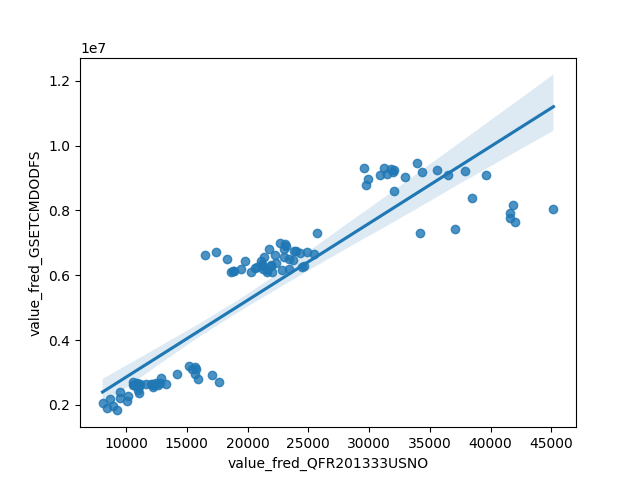
\includegraphics[scale = 0.9]{plots/plot_2026-10-14.png}
\caption{Raw Regression Plot for 2026-10-14}
\end{figure}
\newpage
\subsection{Detrended Regression}
\noindent Regresses the residuals of each series after removing its own linear time trend, so a shared trend can no longer drive the result on its own. A relationship that stays significant here is better evidence of a genuine link between the two series.

\begin{center}
\begin{tabular}{lclc}
\toprule
\textbf{Dep. Variable:}                        & value\_fred\_GSETCMDODFS\_detrended & \textbf{  R-squared:         } &     0.022   \\
\textbf{Model:}                                &                 OLS                 & \textbf{  Adj. R-squared:    } &     0.013   \\
\textbf{Method:}                               &            Least Squares            & \textbf{  F-statistic:       } &     2.317   \\
\textbf{Date:}                                 &           Wed, 14 Oct 2026          & \textbf{  Prob (F-statistic):} &    0.131    \\
\textbf{Time:}                                 &               16:02:51              & \textbf{  Log-Likelihood:    } &   -1530.9   \\
\textbf{No. Observations:}                     &                   103               & \textbf{  AIC:               } &     3066.   \\
\textbf{Df Residuals:}                         &                   101               & \textbf{  BIC:               } &     3071.   \\
\textbf{Df Model:}                             &                     1               & \textbf{                     } &             \\
\textbf{Covariance Type:}                      &              nonrobust              & \textbf{                     } &             \\
\bottomrule
\end{tabular}
\begin{tabular}{lcccccc}
                                               & \textbf{coef} & \textbf{std err} & \textbf{t} & \textbf{P$> |$t$|$} & \textbf{[0.025} & \textbf{0.975]}  \\
\midrule
\textbf{const}                                 &   -4.732e-09  &     6.86e+04     &  -6.9e-14  &         1.000        &    -1.36e+05    &     1.36e+05     \\
\textbf{value\_fred\_QFR201333USNO\_detrended} &      28.1415  &       18.489     &     1.522  &         0.131        &       -8.536    &       64.819     \\
\bottomrule
\end{tabular}
\begin{tabular}{lclc}
\textbf{Omnibus:}       & 13.571 & \textbf{  Durbin-Watson:     } &    0.344  \\
\textbf{Prob(Omnibus):} &  0.001 & \textbf{  Jarque-Bera (JB):  } &   16.691  \\
\textbf{Skew:}          &  0.705 & \textbf{  Prob(JB):          } & 0.000237  \\
\textbf{Kurtosis:}      &  4.378 & \textbf{  Cond. No.          } & 3.71e+03  \\
\bottomrule
\end{tabular}
%\caption{OLS Regression Results}
\end{center}

Notes: \newline
 [1] Standard Errors assume that the covariance matrix of the errors is correctly specified. \newline
 [2] The condition number is large, 3.71e+03. This might indicate that there are \newline
 strong multicollinearity or other numerical problems.

\begin{figure}
\centering
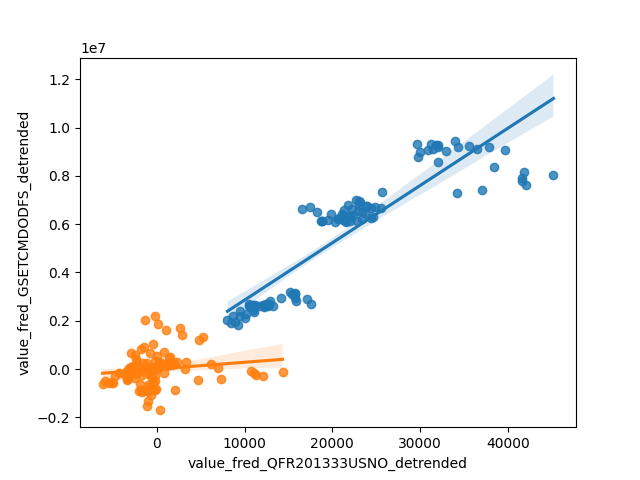
\includegraphics[scale = 0.9]{plots/plot_2026-10-14_detrended.png}
\caption{Detrended Regression Plot for 2026-10-14}
\end{figure}
\newpage
